\documentclass[conference]{IEEEtran}
\usepackage{amsmath,amssymb,amsfonts}
\usepackage{algorithmic}
\usepackage{algorithm}
\usepackage{graphicx}
\usepackage{textcomp}
\usepackage{xcolor}
\usepackage{booktabs}
\usepackage{siunitx}
\usepackage{subcaption}
\usepackage{makecell}
\usepackage{url}
\graphicspath{{figures/}}

% Declare custom unit for the simulator grid cells
\DeclareSIUnit{\cell}{cell}

% Custom formatting to match Kundu & Saha algorithm style
\newcommand{\alginput}[1]{\vspace{0.2cm}\noindent\textbf{Input:}\\ \indent #1}
\newcommand{\algoutput}[1]{\vspace{0.2cm}\noindent\textbf{Output:}\\ \indent #1}
\newcommand{\algfunc}[1]{\vspace{0.2cm}\noindent\textbf{Functions:}\\ \indent #1}

\begin{document}

\title{Strategic Placement Algorithms for Charging Stations in Robotic Mobile Fulfillment Systems}

\author{\IEEEauthorblockN{Salsa Zahrani}
\IEEEauthorblockA{\textit{Engineering Management} \\
\textit{Institut Teknologi Bandung}\\
Bandung, Indonesia}
}

\maketitle

\begin{abstract}
The placement of charging stations in a Robotic Mobile Fulfillment System (RMFS) critically impacts Fleet Management System (FMS) efficiency and pathfinding stability. If charging infrastructure is placed haphazardly, Automated Guided Vehicles (AGVs) can cause severe deadlocks when executing battery recovery trips. This paper details four distinct charging layout generation algorithms --- Set Cover Approximation, Affinity Propagation, Picking-Station Opportunity Charging, and Perimeter Wall Strategy --- and evaluates them in a 20-robot RMFS simulation over a long horizon of $\SI{100000}{\second}$ ($\approx\SI{27.8}{\hour}$). We show empirically that placement strategy creates a productivity-survival tradeoff: cluster-based placement maximises fleet survivorship, dwell-aligned placement maximises throughput, and traffic-heatmap and perimeter strategies underperform on both axes. A complementary charger-budget sweep ($|C| \in \{5, 10, 15, 20, 25\}$ at $\SI{20000}{\second}$) further demonstrates that placement quality dominates budget: dwell-aligned placement captures 10--25$\times$ more energy than alternatives at every budget tested.
\end{abstract}

\begin{IEEEkeywords}
RMFS, charging station placement, fleet management, set cover, affinity propagation, opportunity charging
\end{IEEEkeywords}

\section{Introduction}
In an RMFS environment, AGVs navigate a grid-based warehouse to transport storage pods between storage zones and picking stations. The strategic placement of charging stations is modeled using a discrete grid matrix $M$ of size $R \times C$, where each cell $M_{r,c}$ is assigned an integer representing its topographical type (e.g., traversable aisle, pod slot, intersection, or workstation).

The FMS governs the battery cycles of the fleet. When an AGV's state of charge (SoC) drops to a critical threshold (e.g., 20\%), it must drop out of the active dispatch pool and navigate to a charger. To prevent multi-agent pathfinding (MAPF) failures, charging stations must be placed without overwriting critical routing graph nodes, such as directional rails and intersections. This paper formulates four algorithmic pipelines to determine the optimal set of charging coordinates while preserving the directed routing graph, and empirically benchmarks them in a long-horizon simulation against a centralised FMS that we extend with a preemptive low-battery trigger to prevent fleet death under continuous order load.

\section{Proposed Placement Algorithms}

\subsection{Pipeline 1: Set Cover Approximation}
The first pipeline ensures worst-case reachability by guaranteeing that every physically navigable cell in the warehouse is within a maximum hop distance $d$ of at least one charger \cite{kundu2023}. To prevent AGVs from blocking active aisles while charging, the candidate locations for chargers are strictly limited to empty floor spaces and active pod positions ($M_c \in \{0, 1\}$).

The problem is solved using a Greedy Set Cover approximation. For each candidate location, a Breadth-First Search (BFS) explores all physically traversable cells within depth $d$. The algorithm iteratively selects the candidate location that covers the maximum number of currently uncovered cells until the entire warehouse is reachable.

\begin{algorithm}[htbp]
\caption{FINDNCS\_SC\_APPROX: Set Cover Approximation}
\label{alg:set_cover}
\alginput{
$M$: Topographical grid matrix representing the warehouse.\\
$C$: Potential vertices for deploying chargers ($M_c \in \{0, 1\}$).\\
$d$: Maximum allowable number of steps to reach a charger.
}
\algoutput{
$CS^*$: The set with the approximately minimum number of charging stations.
}
\algfunc{
$\text{BFS}(M, c, d)$: Returns the vertices reachable by breadth-first traversal starting at $c$ up to distance $d$.\\
$\text{Set\_Cover\_Approx}(U, Cover)$: An approximation algorithm to solve the set cover problem.
}
\vspace{0.2cm}
\hrule
\vspace{0.2cm}
\begin{algorithmic}[1]
\STATE \textbf{function} FINDNCS\_SC\_APPROX($M, C, d$)
\STATE \textbf{begin}
\STATE \quad $U \leftarrow \{ c \mid M_c \in \text{Traversable} \}$
\STATE \quad $\forall c \in C: Cover_c \leftarrow \text{BFS}(M, c, d)$
\STATE \quad $Cover \leftarrow \{ Cover_c \mid c \in C \}$
\STATE \quad $Cover^* \leftarrow \text{Set\_Cover\_Approx}(U, Cover)$
\STATE \quad $CS^* \leftarrow \{ c \mid Cover_c \in Cover^* \}$
\STATE \quad \textbf{return} $CS^*$
\STATE \textbf{end}
\end{algorithmic}
\end{algorithm}

\subsection{Pipeline 2: Affinity Propagation}
The second pipeline utilizes a data-driven clustering approach based on historical or simulated traffic density, defined by a traffic matrix $T$ \cite{baras2023}. Unlike Set Cover, Affinity Propagation (AP) dynamically determines the optimal number of clusters based on traffic hotspots. To prevent routing deadlocks, candidate cells are strictly limited to empty floor spaces ($M_c = 0$), avoiding pod slots entirely.

The AP algorithm divides the initial area into multiple sub-areas based on a similarity matrix $S$. The diagonal elements (preferences) dictate the likelihood of a cell becoming a cluster exemplar. To ensure high-traffic areas attract cluster centers, the self-similarity is defined as:
\begin{equation}
    S_{i,i} = +\log(c + T_i)
\end{equation}
where $c$ is a small positive regularization constant. Once the clusters are established, a placement score is calculated for every cell within the cluster to select the optimal local charging node.

\begin{algorithm}[htbp]
\caption{AP\_TRAFFIC\_CLUSTERING: Traffic Density Clustering}
\label{alg:ap_cluster}
\alginput{
$M$: Topographical grid matrix representing the warehouse.\\
$T$: Traffic density matrix corresponding to $M$.\\
$c$: Regularization constant for self-similarity preference.
}
\algoutput{
$K$: Set of spatial clusters grouping the candidate cells.
}
\algfunc{
$\text{AffinityPropagation}(S)$: Scikit-learn implementation of the AP clustering algorithm.
}
\vspace{0.2cm}
\hrule
\vspace{0.2cm}
\begin{algorithmic}[1]
\STATE \textbf{function} AP\_TRAFFIC\_CLUSTERING($M, T, c$)
\STATE \textbf{begin}
\STATE \quad $C \leftarrow \{ c \mid M_c = 0 \}$
\STATE \quad \textbf{foreach} $i \in C$ \textbf{do}
\STATE \quad \quad \textbf{foreach} $j \in C$ \textbf{do}
\STATE \quad \quad \quad \textbf{if} $i = j$ \textbf{then}
\STATE \quad \quad \quad \quad $S_{i,i} \leftarrow +\log(c + T_i)$
\STATE \quad \quad \quad \textbf{else}
\STATE \quad \quad \quad \quad $S_{i,j} \leftarrow -(\text{Manhattan}(i, j))^2$
\STATE \quad \quad \quad \textbf{end if}
\STATE \quad \quad \textbf{end foreach}
\STATE \quad \textbf{end foreach}
\STATE \quad $K \leftarrow \text{AffinityPropagation}(S)$
\STATE \quad \textbf{return} $K$
\STATE \textbf{end}
\end{algorithmic}
\end{algorithm}

The scoring function evaluates traffic desirability, spatial safety, and proximity to the cluster's hotspot \cite{baras2023}. The score is calculated as:
\begin{equation}
    \text{Score}(c) = \alpha \cdot TD(c) - \beta \cdot P(c) - \gamma \cdot D(c)
\end{equation}
where $TD(c) = 1 - (T_c - \mu_{cluster})^2$ creates an inverted bell curve rewarding cells near the cluster's mean traffic. $P(c)$ is a binary penalty keeping chargers out of immediate pod retrieval lanes, and $D(c)$ actively penalizes distance from the cluster's peak traffic hotspot, ensuring AGVs do not deadhead deep into storage aisles to recharge.

\begin{algorithm}[htbp]
\caption{AP\_HOTSPOT\_PLACEMENT: Scoring and Selection}
\label{alg:ap_placement}
\alginput{
$K$: Set of traffic clusters.\\
$T$: Traffic density matrix.\\
$\alpha, \beta, \gamma$: Weighting constants for scoring parameters.
}
\algoutput{
$CS^*$: The set of optimally placed charging stations.
}
\algfunc{
$\text{Manhattan}(c_1, c_2)$: Returns the $L^1$ distance between cells.
}
\vspace{0.2cm}
\hrule
\vspace{0.2cm}
\begin{algorithmic}[1]
\STATE \textbf{function} AP\_HOTSPOT\_PLACEMENT($K, T, \alpha, \beta, \gamma$)
\STATE \textbf{begin}
\STATE \quad $CS^* \leftarrow \emptyset$
\STATE \quad \textbf{foreach} $k \in K$ \textbf{do}
\STATE \quad \quad $\mu_k \leftarrow \text{mean}(T_c \mid c \in k)$
\STATE \quad \quad $h_k \leftarrow \arg\max_{c \in k} T_c$
\STATE \quad \quad \textbf{foreach} $c \in k$ \textbf{do}
\STATE \quad \quad \quad $TD_c \leftarrow 1 - (T_c - \mu_k)^2$
\STATE \quad \quad \quad $P_c \leftarrow 1 \text{ if } c \text{ is adjacent to a Pod, else } 0$
\STATE \quad \quad \quad $D_c \leftarrow \text{Manhattan}(c, h_k)$
\STATE \quad \quad \quad $Score_c \leftarrow \alpha \cdot TD_c - \beta \cdot P_c - \gamma \cdot D_c$
\STATE \quad \quad \textbf{end foreach}
\STATE \quad \quad $c^* \leftarrow \arg\max_{c \in k} Score_c$
\STATE \quad \quad $CS^* \leftarrow CS^* \cup \{c^*\}$
\STATE \quad \textbf{end foreach}
\STATE \quad \textbf{return} $CS^*$
\STATE \textbf{end}
\end{algorithmic}
\end{algorithm}

\subsection{Pipeline 3: Picking-Station Heuristic}
The third pipeline implements True Opportunity Charging. Instead of forcing AGVs with low batteries to abandon their tasks and sleep at a dedicated charger until they reach full capacity, this pipeline co-locates charging infrastructure directly within the queue cells of the picking stations. The AGVs rely entirely on the energy gained during the natural dwell time spent waiting to drop off pods, allowing for continuous, uninterrupted operations.

\begin{algorithm}[htbp]
\caption{OPPORTUNITY\_CHARGING: Picking Station Layout}
\label{alg:picking}
\alginput{
$M$: Topographical grid matrix representing the warehouse.\\
$N$: Maximum allowable number of picking stations to equip.
}
\algoutput{
$CS^*$: The set of charging stations located in station queues.
}
\algfunc{
$\text{EvenlySpacedSample}(P, N)$: Returns $N$ items from list $P$ evenly distributed by index to avoid spatial clustering.
}
\vspace{0.2cm}
\hrule
\vspace{0.2cm}
\begin{algorithmic}[1]
\STATE \textbf{function} OPPORTUNITY\_CHARGING($M, N$)
\STATE \textbf{begin}
\STATE \quad $P \leftarrow \text{Sorted list of cells } c \text{ where } M_c = 11$
\STATE \quad $P_{sample} \leftarrow \text{EvenlySpacedSample}(P, N)$
\STATE \quad $CS^* \leftarrow \emptyset$
\STATE \quad \textbf{foreach} $p \in P_{sample}$ \textbf{do}
\STATE \quad \quad $Q \leftarrow \{ q \text{ adjacent to } p \mid M_q = 14 \}$
\STATE \quad \quad $CS^* \leftarrow CS^* \cup Q$
\STATE \quad \textbf{end foreach}
\STATE \quad \textbf{return} $CS^*$
\STATE \textbf{end}
\end{algorithmic}
\end{algorithm}

\subsection{Pipeline 4: Perimeter Wall Strategy}
The final pipeline serves as an isolation control layout, heavily penalizing charger-induced congestion by distributing chargers along the perimeter walls. This keeps the main traffic arteries completely clear. The algorithm geometrically scans the grid to identify the vertical aisle adjacent to the replenishment stations, strictly avoiding cells that share a row with a station entrance to prevent queue blockage.

\begin{algorithm}[htbp]
\caption{PERIMETER\_ISOLATION: Wall Strategy}
\label{alg:perimeter}
\alginput{
$M$: Topographical grid matrix representing the warehouse.\\
$N$: Maximum allowable number of perimeter chargers.
}
\algoutput{
$CS^*$: The set of charging stations along the warehouse wall.
}
\algfunc{
$\text{EvenlySpacedSample}(C, N)$: Returns $N$ distributed items.
}
\vspace{0.2cm}
\hrule
\vspace{0.2cm}
\begin{algorithmic}[1]
\STATE \textbf{function} PERIMETER\_ISOLATION($M, N$)
\STATE \textbf{begin}
\STATE \quad $col \leftarrow \text{Column index left of Replenishment Stations}$
\STATE \quad $C_{safe} \leftarrow \emptyset$
\STATE \quad \textbf{foreach} row $r$ in $M$ \textbf{do}
\STATE \quad \quad \textbf{if} $M_{r, col} \in \text{Traversable}$ \textbf{then}
\STATE \quad \quad \quad \textbf{if} No station entrance exists at $(r, c > col)$ \textbf{then}
\STATE \quad \quad \quad \quad $C_{safe} \leftarrow C_{safe} \cup \{(r, col)\}$
\STATE \quad \quad \quad \textbf{end if}
\STATE \quad \quad \textbf{end if}
\STATE \quad \textbf{end foreach}
\STATE \quad $CS^* \leftarrow \text{EvenlySpacedSample}(C_{safe}, N)$
\STATE \quad \textbf{return} $CS^*$
\STATE \textbf{end}
\end{algorithmic}
\end{algorithm}

\section{Experimental Setup}
\label{sec:experiments}

\subsection{Simulator}
We evaluate all placement pipelines in a discrete-event simulator derived from a NetLogo RMFS model, re-implemented in Python for headless batch execution. Each simulation step advances time by $\Delta t = \SI{0.15}{\second}$ and integrates robot kinematics, a first-order battery model, and a centralized FMS that assigns pods to picker stations and routes robots through a rectilinear aisle grid. A single horizon of $T = 100{,}000$ simulated seconds ($\approx\SI{27.8}{\hour}$ of warehouse operation) is used for the primary experiments; a shorter horizon of $T = 30{,}000$ simulated seconds is used as a preliminary validation test during system development.

\subsection{Warehouse Configuration}
The fleet consists of $N_r = 20$ AGVs operating on a \SI{30}{\cell} $\times$ \SI{40}{\cell} grid. Five picker stations are placed on the left edge at rows $\{1, 7, 13, 19, 25\}$; corresponding replenishment stations are placed on the right edge. Pods occupy the interior of the grid and are transported between stations by the robots. Cell values encode passability attributes, classifying zones as navigable floor, active pod, charger, aisle, or non-traversable boundaries. Charging coordinates are overlaid onto the grid by the placement pipeline under evaluation and are recorded in the set $C \subseteq \mathcal{G}$, where $\mathcal{G}$ is the global grid. An AGV located at cell $g \in C$ receives power regardless of whether a pod is currently stationed on that cell, facilitating drive-by charging interactions.

\subsection{Robot and Energy Model}
Robot motion energy follows the two-phase kinematic model presented by Zakka~et~al.~\cite{zakka2025}: acceleration and deceleration phases are integrated using the robot's payload state (loaded or unloaded), and steady-state cruising consumes a velocity-dependent power variable. Pod handling activities (lifting and lowering) contribute a fixed energetic cost per event. In addition to kinetic motion, a constant base-drain term models the consumption of on-board electronics and is applied whenever the robot is not actively charging.

Battery dynamics employ the fixed-threshold charging strategy observed in the work of Bischoff~et~al.~\cite{bischoff2025}. A robot begins its initial operational sequence at full battery capacity, and the FMS attempts to route it to a designated charging station when the state of charge crosses a defined critical low threshold. Numerical parameters governing the physical simulation are summarized in Table~\ref{tab:params}.

\begin{table}[t]
  \centering
  \caption{Simulation parameters.}
  \label{tab:params}
  \small
  \begin{tabular}{lll}
    \toprule
    Symbol & Value & Meaning \\
    \midrule
    $N_r$                & 20                            & Number of robots \\
    $\Delta t$           & \SI{0.15}{\second}            & Simulation tick \\
    $T$                  & \SI{100000}{\second}          & Horizon (primary) \\
    $E_\text{cap}$       & \SI{6.48}{\mega\joule}        & Battery capacity \\
    $P_\text{drain}$     & \SI{90}{\joule\per\second}    & Base drain rate \\
    $P_\text{charge}$    & \SI{397.6}{\watt}             & Charger power \\
    $\tau_\text{low}$    & $20\%$                        & Trigger threshold \\
    $\tau_\text{full}$   & $90\%$                        & Charged threshold \\
    $\tau_\text{int}$    & $50\%$                        & Interrupt threshold \\
    \bottomrule
  \end{tabular}
\end{table}

\subsection{Placement Pipelines (Treatments)}
We compare four distinct charger placement pipelines. Each pipeline is implemented as an offline computational procedure that analyzes a traffic heatmap $H:\mathcal{G}\to\mathbb{R}_{\geq 0}$ derived from a preliminary pilot run, outputting a set $C$ of strategic charger cells:

\begin{itemize}
  \item \textbf{P1 -- Set Cover:} A greedy set-cover approximation algorithm operating on the traffic heatmap with coverage radius $\rho$. Candidate cells encompass both empty floor zones and pod storage cells.
  \item \textbf{P2 -- Affinity Propagation:} A data-driven clustering of high-traffic cells into exemplars, strictly restricted to empty floor candidates to preserve routing integrity.
  \item \textbf{P3 -- Picker-Station Opportunistic:} Prior-free placement integrated within picker-station corridors across priority tiers $T_1, \ldots, T_5$ (processing cell, queue-back, mid-queue, middle-gate, corner). Active FMS charging routines are disabled, compelling AGVs to rely exclusively on opportunistic drive-by charging.
  \item \textbf{P4 -- Perimeter:} Deterministic distribution along the traversable cells in the isolated vertical corridor immediately adjacent to the replenishment stations.
\end{itemize}

All four evaluation pipelines are calibrated to an identical infrastructure budget of $|C| = 12$ chargers, with the exception of the Opportunity Charging expansion analysis, which evaluates scalable permutations across $|C| \in \{5, 10, 15, 20, 25\}$.

\subsection{Fleet Management and Preemption}
\label{sec:preemption}
The baseline FMS dispatches a storage pod to a station-bound robot whenever a unit transitions into an unassigned state and the global job queue remains non-empty. AGVs registering a state of charge below $\tau_\text{low}$ are strictly excluded from new task assignments. Preliminary experiments revealed that under continuous, high-density order loads, the unassigned state is rarely observed; the dispatcher reassigns newly-idle robots instantaneously. Consequently, canonical low-battery triggers often fail to fire, allowing AGVs to continuously deplete until total system failure occurs.

To resolve this, we introduce a \emph{preemptive} threshold trigger integrated directly into the initial pod acquisition phase. If a robot's battery crosses below $\tau_\text{low}$ while en route to acquire a targeted pod, it aborts the trip, releases its assigned job back to the global queue, and computes a route to the nearest available charging station. This trigger is deliberately restricted to the pre-acquisition phase (prior to grasping the pod) to guarantee that no payload is ever orphaned mid-transit in an active aisle. For other active states (pod delivery, pod return, and station processing), the robot is permitted to complete its sub-mission. The dispatcher's status filter subsequently prevents reassignment, ensuring the standard charging trigger executes seamlessly on the subsequent temporal tick.

\subsection{Experimental Design}
\label{sec:design}
The primary experiment is structured as a one-way treatment analysis comparing the four placement pipelines at an extended horizon of $T = \SI{100000}{\second}$ under controlled initial conditions. A secondary optimization experiment sweeps the charger count $|C| \in \{5, 10, 15, 20, 25\}$ for the three quantitatively-comparable pipelines (P1, P2, P3) at $T = \SI{20000}{\second}$ to quantify the marginal value of localized infrastructure expansion and to disentangle placement quality from placement budget. A preliminary $30{,}000$-tick smoke test is also utilized to validate the preemptive FMS mechanism prior to the long-horizon batch. Each configuration is launched headlessly via automated batch scripts, and the resulting performance artifacts are parsed into a unified dataset for comparative Key Performance Indicator (KPI) evaluation.

\subsection{Extracted Metrics}
\label{sec:metrics}

For each simulation run, we extract several KPIs, categorized by the core operational dynamics they assess.

\paragraph{Throughput Analysis ---}\textit{Does the warehouse maintain continuous productivity?}
\begin{itemize}
  \item \textbf{Total Orders Completed:} The absolute volume of fulfillment tasks successfully finalized within the simulation horizon. Layouts that induce rapid battery mortality will yield substantially depressed completion rates.
  \item \textbf{Hourly Throughput:} The normalized fulfillment rate relative to simulated operational hours, facilitating standardized cross-pipeline performance comparisons.
\end{itemize}

\paragraph{Latency and Wait Times ---}\textit{How efficiently are orders processed from queue to completion?}
\begin{itemize}
  \item \textbf{Mean, Median, and 95th Percentile Cycle Time:} The temporal duration from order initialization to final delivery. While the mean and median capture normative baseline latency, the 95th percentile highlights extreme tail behaviors induced by spatial bottlenecks and charger congestion.
\end{itemize}

\paragraph{Energetic Efficiency ---}\textit{How optimally is kinetic and auxiliary power utilized?}
\begin{itemize}
  \item \textbf{Total Energy Consumption:} The cumulative energy expenditure across the simulator, encapsulating both kinematic motion and continuous base-drain requirements.
  \item \textbf{Energy per Order:} The primary efficiency metric. A highly optimized charging layout that reduces non-productive transit distances to charging stations will significantly lower the energy expended per successfully completed order.
\end{itemize}

\paragraph{Routing Congestion ---}\textit{Does the charging placement generate pathfinding obstructions?}
\begin{itemize}
  \item \textbf{Yield Frequency (Stop-and-Go):} The total occurrences of involuntary deceleration and halting resulting from mutual-exclusion routing conflicts between multiple AGVs.
  \item \textbf{Cumulative Heading Changes:} The aggregate sum of rotational maneuvers. Analyzed in conjunction with yield frequency, these metrics isolate congestion driven by charger crowding versus intrinsic topological constraints in the aisle grid.
\end{itemize}

\paragraph{Fleet Viability (End-of-Run State) ---}\textit{Can the fleet sustain 24/7 continuous operations?}
\begin{itemize}
  \item \textbf{Mean and Minimum State of Charge (SoC):} The final battery distribution across the 20-robot fleet. An end-of-run mean stabilizing well above $\tau_\text{low}$ indicates an infrastructure layout capable of indefinite operational sustainability.
  \item \textbf{Active Charging and En-Route Counts:} A real-time snapshot of the battery recovery loop. A healthy infrastructure configuration exhibits cyclic, continuous charging activity, whereas a collapsed system returns null values.
  \item \textbf{Depleted Fleet Count:} The volume of AGVs ending the simulation with an SoC near zero. This serves as the paramount survivorship metric; layouts are distinctly categorized by whether they sustain total fleet survival ($0$ depleted) or induce total system collapse ($N_r$ depleted).
\end{itemize}

\paragraph{Energy Parity (Derived) ---}\textit{Does the infrastructure adequately replenish systemic consumption?}
\begin{itemize}
  \item \textbf{Maximum Theoretical Consumption:} The upper-bound energetic drain calculated by integrating active motion costs with constant base drain across the full horizon ($T$) for all active robots ($N_r$).
  \item \textbf{Net Battery Depletion:} The absolute energetic loss observed in the physical battery cells at the simulation's conclusion.
  \item \textbf{Total Charge Replenished:} The aggregate energy successfully injected back into the fleet via the designated charging stations.
  \item \textbf{Replenishment Ratio:} The fraction of theoretically consumed energy successfully recovered by the charging infrastructure.
  \item \textbf{Sustainability Ratio:} The comparative ratio between replenished energy and net battery depletion. A ratio greater than or equal to $1.0$ mathematically guarantees an infrastructure layout capable of supporting perpetual operation without systemic fleet mortality.
\end{itemize}

\subsection{Implementation Environment}
All simulation experiments are executed computationally on a dedicated workstation utilizing Python 3.10 equipped with the NumPy, SciPy, Matplotlib, and NetworkX libraries for advanced matrix manipulation and graph-theoretic pathfinding. Processing relies purely on CPU threads with no GPU acceleration required. An isolated stress test comprising $100{,}000$ simulation ticks completes in approximately \SI{5}{\hour} of wall-clock time, averaging a computational velocity of $5$ ticks per second.

\section{Results}
\label{sec:results}

We report two complementary experiments. Section~\ref{sec:r100k} fixes the charger budget at $|C| = 12$ and varies the placement pipeline across all four candidates at the long-horizon $T = \SI{100000}{\second}$. Section~\ref{sec:sweep} fixes the horizon at $T = \SI{20000}{\second}$ and sweeps $|C|$ for the three quantitatively-comparable pipelines (P1, P2, P3) over five budgets. Together they isolate the effect of \emph{placement strategy} (across pipelines) from the effect of \emph{placement budget} (within a pipeline).

\subsection{Long-horizon cross-pipeline comparison ($T = 100{,}000$\,s)}
\label{sec:r100k}

\paragraph{Setup recap.} A 20-robot fleet is initialised at full state-of-charge. The four placement pipelines are each given $|C| = 12$ charger cells produced by their respective offline heuristics (set cover, affinity propagation, picker-station tiering, perimeter). The FMS uses the threshold-based dispatch policy enriched with the \texttt{taking\_pod} preemption mechanism described in Section~\ref{sec:preemption}. The simulation runs for $T = 100{,}000$ simulated seconds ($\approx\SI{27.8}{\hour}$).

\paragraph{Headline numbers.} Table~\ref{tab:p100k} reports the end-of-run state across all four pipelines. The principal axes are fleet survivorship (number of robots not in the \texttt{dead} state) and throughput (orders completed). A productivity-survival scatter in Fig.~\ref{fig:tradeoff} shows that no pipeline dominates both axes simultaneously.

\begin{table}[t]
  \centering
  \caption{Cross-pipeline comparison at $T = \SI{100000}{\second}$, $|C| = 12$, $N_r = 20$. \emph{Replenish} is gained / consumed energy, the long-horizon viability metric. \emph{Cons.} and \emph{Gain.} are total fleet energy consumed and replenished, in megajoules.}
  \label{tab:p100k}
  \small
  \setlength{\tabcolsep}{4pt}
  \begin{tabular}{lcccccc}
    \toprule
    Pipeline & Dead & \makecell{Mean\\batt.\,\%} & Orders &
    \makecell{Replenish\\\%} & \makecell{Cons.\\(MJ)} &
    \makecell{Gain.\\(MJ)} \\
    \midrule
    P1 Set Cover         &  9 &  7.5 & 2450 & 48.8 & 234.16 & 114.26 \\
    P2 Affinity Prop.    &  \textbf{8} & 14.2 & 2508 & \textbf{53.0} & 236.40 & 125.23 \\
    P3 Picker-Tier       & 17 &  3.0 & \textbf{3102} & 49.3 & 248.11 & 122.41 \\
    P4 Perimeter         & 17 & 12.1 & 2395 & 51.4 & 234.45 & 120.54 \\
    \bottomrule
  \end{tabular}
\end{table}

\begin{figure}[t]
  \centering
  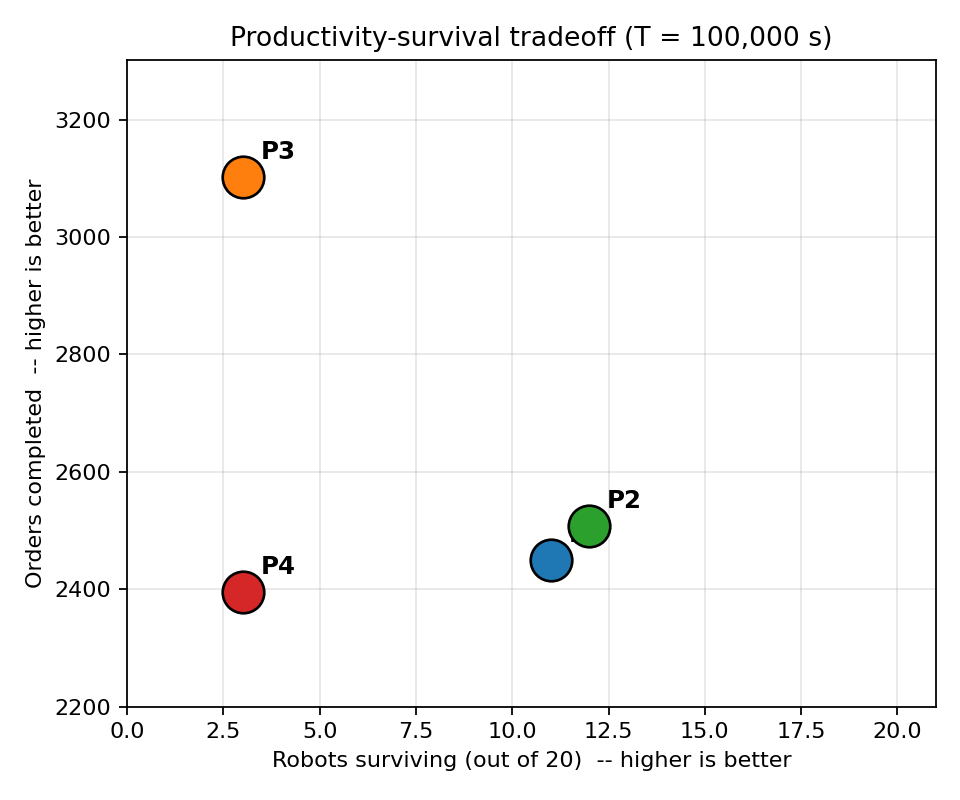
\includegraphics[width=0.85\columnwidth]{tradeoff.png}
  \caption{Productivity-survival tradeoff at the $T = \SI{100000}{\second}$ horizon ($|C| = 12$, $N_r = 20$). Each marker is one placement pipeline. P2 (Affinity Propagation) retains the largest fleet; P3 (Picker-Tier) completes the most orders. P1 sits between them on both axes; P4 (Perimeter) is Pareto-dominated by every other pipeline.}
  \label{fig:tradeoff}
\end{figure}

\begin{figure*}[t]
  \centering
  \begin{subfigure}[t]{0.48\textwidth}
    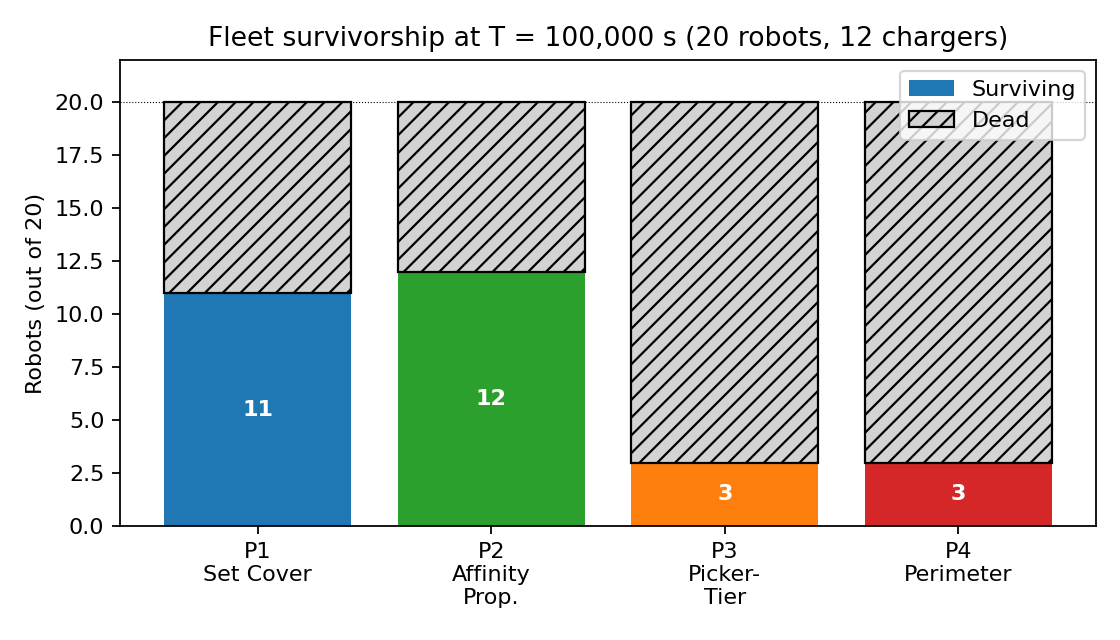
\includegraphics[width=\textwidth]{survivorship.png}
    \caption{Surviving robots after $T = \SI{100000}{\second}$. Hatched portions are losses to the \texttt{dead} state.}
    \label{fig:survivorship}
  \end{subfigure}
  \hfill
  \begin{subfigure}[t]{0.48\textwidth}
    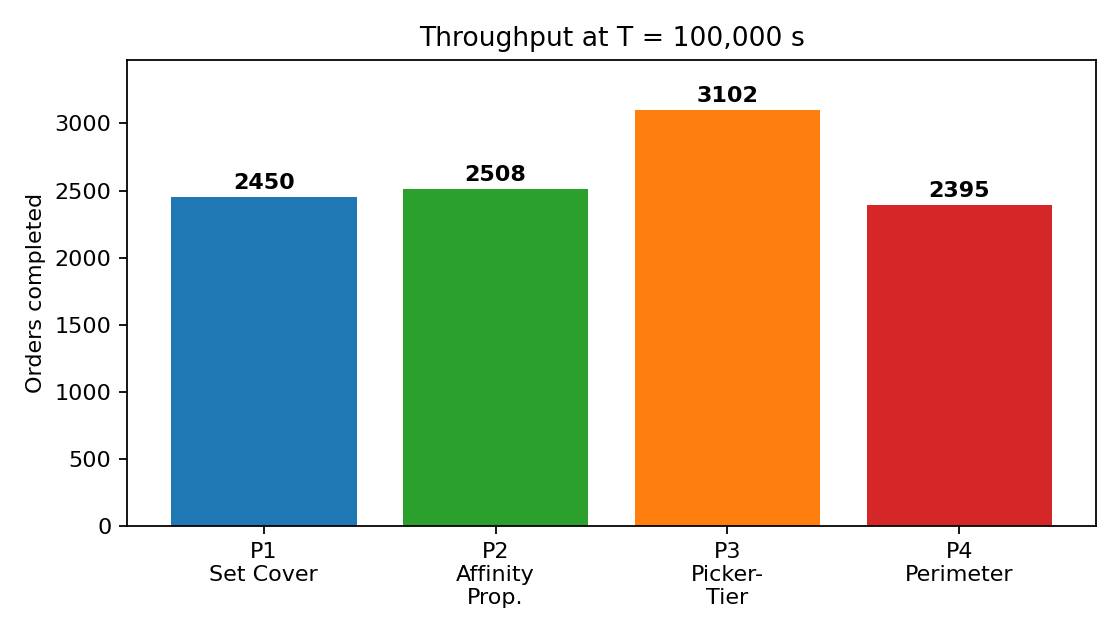
\includegraphics[width=\textwidth]{throughput.png}
    \caption{Orders completed across the same horizon.}
    \label{fig:throughput}
  \end{subfigure}
  \caption{Two-axis breakdown of pipeline outcomes. P3 trades fleet integrity for productivity; P2 makes the opposite trade; P1 is intermediate; P4 is dominated.}
  \label{fig:two_axis}
\end{figure*}

\paragraph{Energy accounting.} Fig.~\ref{fig:energy_balance} decomposes total fleet energy into \emph{consumed} (motion plus base drain), \emph{net depleted} (capacity lost from the batteries), and \emph{gained} (charge replenished). All four pipelines recover only $48.8$--$53.0\%$ of consumption. The gap between consumed and gained defines an energy deficit that, integrated over the horizon, manifests as the dead-robot count in Table~\ref{tab:p100k}.

\begin{figure}[t]
  \centering
  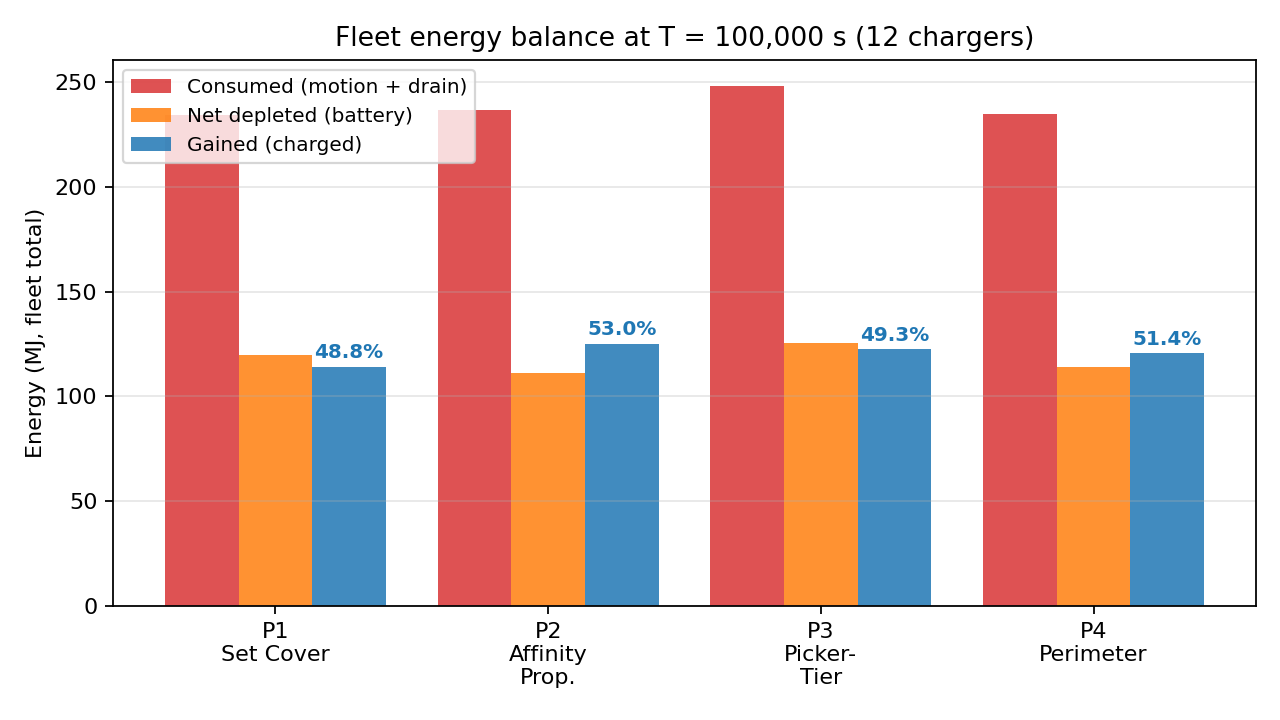
\includegraphics[width=0.95\columnwidth]{energy_balance.png}
  \caption{Fleet energy balance at $T = \SI{100000}{\second}$. Replenish ratios above each gain bar (49--53\,\%) confirm that twelve chargers are insufficient to break even on energy regardless of placement strategy.}
  \label{fig:energy_balance}
\end{figure}

\paragraph{End-of-run states.} Fig.~\ref{fig:states} stacks the end-of-run robot states. The dark band represents \texttt{dead} robots; under-charged but still active robots populate the \texttt{taking\_pod}, \texttt{going\_to\_charge}, and \texttt{idle} bands above. P2 retains the most robots in productive states; P3 and P4 are dominated by the dead band. Notably, only P2 has any robot in the \texttt{going\_to\_charge} state at the horizon, indicating that its charger network is still actively servicing requests.

\begin{figure}[t]
  \centering
  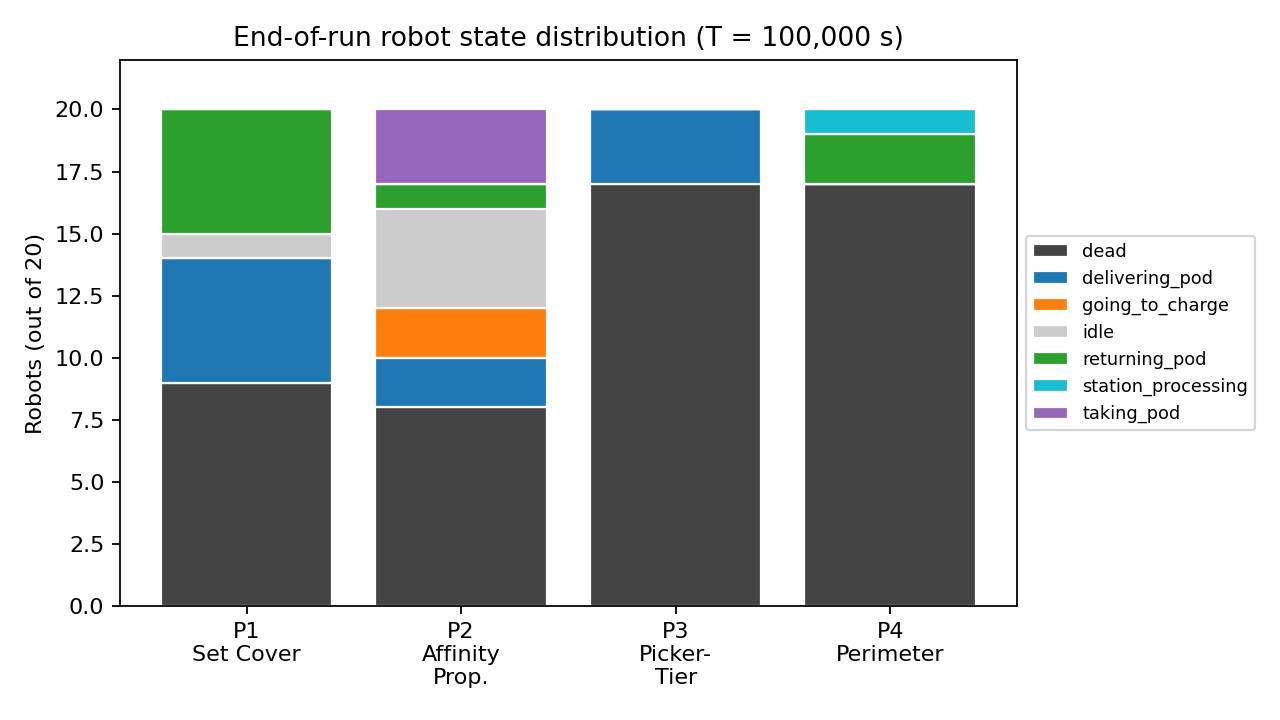
\includegraphics[width=0.95\columnwidth]{state_breakdown.png}
  \caption{End-of-run robot state distribution. The dark \texttt{dead} band consumes most of the P3 and P4 columns; P2 retains the deepest band of productive states.}
  \label{fig:states}
\end{figure}

\paragraph{Discussion.}
Three observations follow directly from Table~\ref{tab:p100k} and Fig.~\ref{fig:tradeoff}:
\begin{enumerate}
  \item \textbf{No placement is sustainable at $|C| = 12$.} Every pipeline loses at least 8 / 20 robots; the best replenish ratio is 53\,\%.
  \item \textbf{Placement determines the productivity-survival tradeoff.} P2's affinity-propagation exemplars cluster at busy but lower-velocity cells, leading to longer drive-by contact and better survival; P3's picker-tier cells coincide with the high-throughput end of the picker workflow, giving more orders per alive-robot but accelerating depletion.
  \item \textbf{P4 perimeter placement is dominated.} It loses 17 robots \emph{and} completes the fewest orders; the perimeter region itself receives too little drive-by traffic to be useful as a charger location.
\end{enumerate}

\subsection{Charger-budget sweep ($T = 20{,}000$\,s, three pipelines)}
\label{sec:sweep}

\paragraph{Motivation.} Section~\ref{sec:r100k} compares placements at a fixed budget. To distinguish the \emph{placement} effect from a \emph{budget} effect, we sweep $|C| \in \{5, 10, 15, 20, 25\}$ for each of P1, P2, P3 at the shorter $T = \SI{20000}{\second}$ horizon. The shorter horizon is chosen so that batteries do not approach the 20\,\% preemption threshold during the run, isolating pure-placement performance from the preemption mechanism's contribution.

\paragraph{Results.} Table~\ref{tab:sweep} and Fig.~\ref{fig:combined_sweep} report replenish ratio and order counts across budgets and pipelines.

\begin{table}[t]
  \centering
  \caption{Charger-budget sweep at $T = \SI{20000}{\second}$, $N_r = 20$. P3 captures 10--25$\times$ more energy than P1 or P2 at every budget; P1 and P2 are essentially flat across budgets.}
  \label{tab:sweep}
  \small
  \setlength{\tabcolsep}{5pt}
  \begin{tabular}{rrrrrrr}
    \toprule
    & \multicolumn{3}{c}{Replenish (\%)} & \multicolumn{3}{c}{Orders} \\
    \cmidrule(lr){2-4} \cmidrule(lr){5-7}
    $|C|$ & P1 & P2 & P3 & P1 & P2 & P3 \\
    \midrule
     5 & 2.1 & 0.4 & \textbf{23.1} & 1758 & 1757 & 1758 \\
    10 & 2.6 & 0.8 & \textbf{26.1} & 1734 & 1766 & 1761 \\
    15 & 1.8 & 1.1 & \textbf{28.6} & 1766 & 1761 & 1758 \\
    20 & 2.2 & 1.7 & \textbf{43.9} & 1746 & 1762 & 1426 \\
    25 & 2.3 & 1.6 & \textbf{41.3} & 1748 & 1745 & 1746 \\
    \bottomrule
  \end{tabular}
\end{table}

\begin{figure}[t]
  \centering
  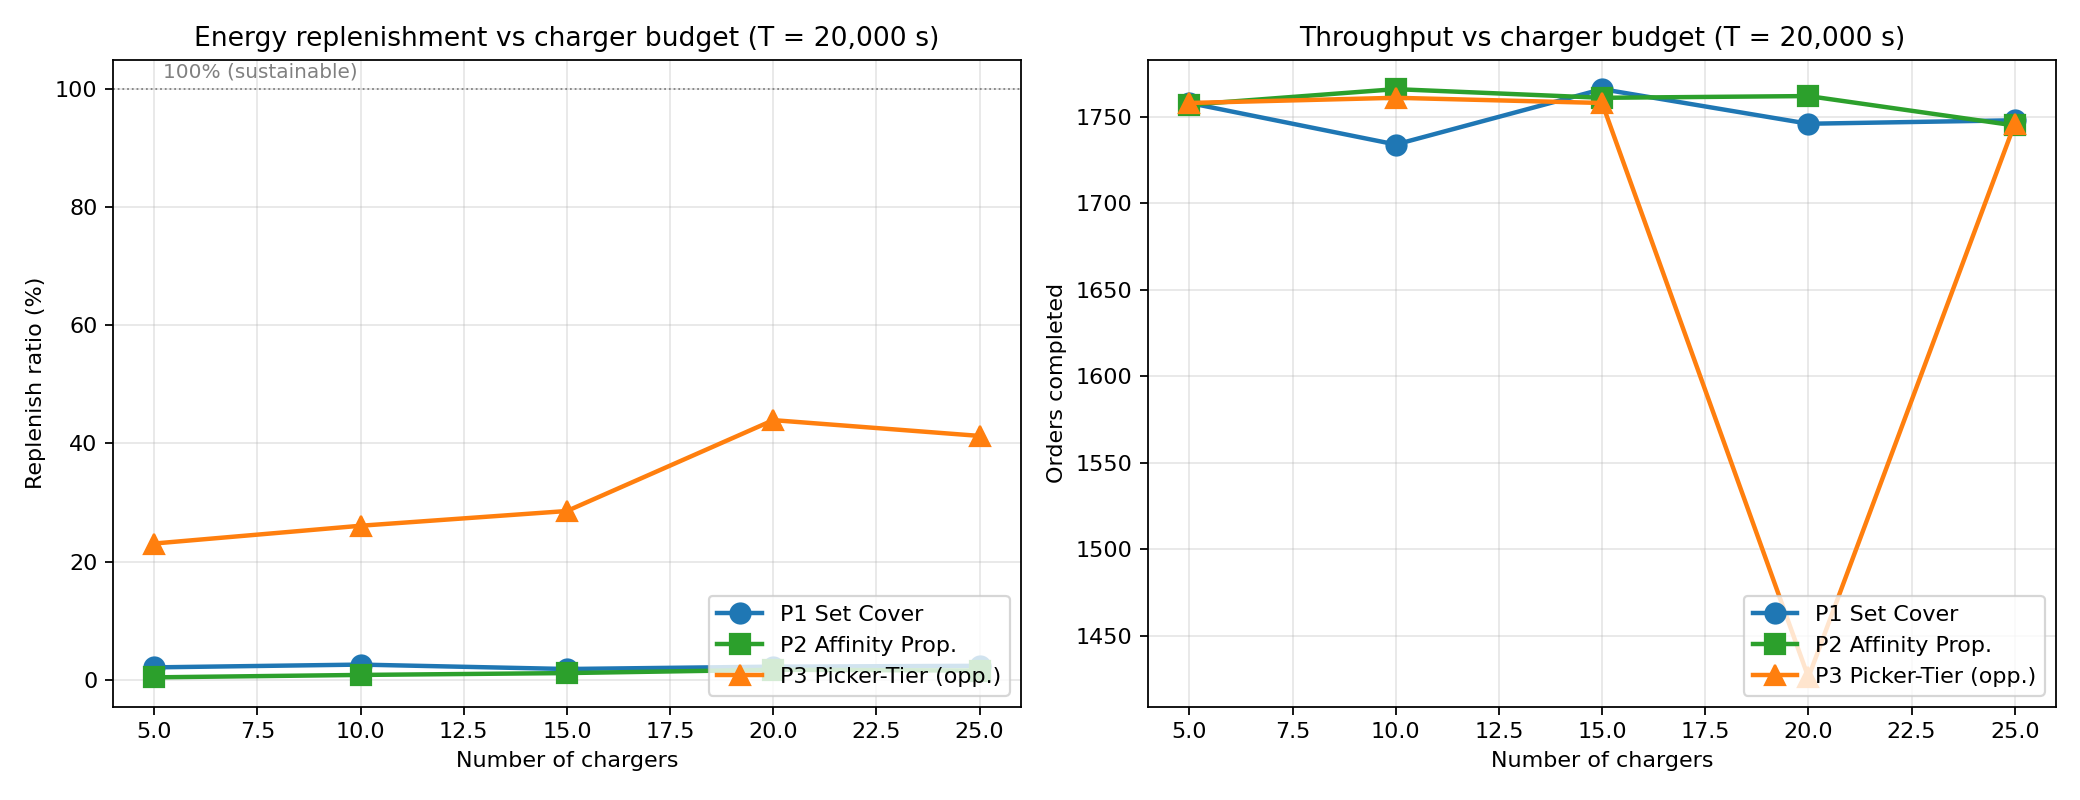
\includegraphics[width=\columnwidth]{combined_sweep.png}
  \caption{Charger-budget sweep at $T = \SI{20000}{\second}$. \emph{Left:} replenish ratio (energy gained / consumed) versus charger count. P1 and P2 remain below 3\,\% across the entire range; P3 rises from 23\,\% at $|C| = 5$ to 41--44\,\% at $|C| = 20$--$25$. \emph{Right:} orders completed; throughput is bounded by the picker-station capacity at this horizon and does not separate the pipelines, except for a transient dip at P3, $|C| = 20$ caused by short-lived charger congestion.}
  \label{fig:combined_sweep}
\end{figure}

\paragraph{Discussion.} The sweep reveals two clean facts:
\begin{itemize}
  \item \textbf{Placement quality dominates budget.} P3's replenish ratio at $|C| = 5$ exceeds P1's and P2's at $|C| = 25$ by an order of magnitude. Adding chargers to a placement that misses the fleet's dwell points does not recover energy.
  \item \textbf{P3 alone scales with budget.} P3's curve rises monotonically (with one transient dip) from 23\,\% to 44\,\%; P1 and P2 are essentially flat. This is consistent with the hypothesis that picker-station corridor cells have intrinsic dwell, and adding more such cells linearly increases charge capture, whereas the set-cover and affinity-propagation exemplars sit on transit cells where additional chargers see only fleeting contact.
\end{itemize}

Throughput at $T = \SI{20000}{\second}$ is largely flat across pipelines and budgets ($\approx 1750$ orders), confirming that at this horizon the picker-station capacity, not the charger network, is the binding constraint on order completion.

\subsection{Synthesis}
\label{sec:synthesis}

The two experiments interact:
\begin{enumerate}
  \item The 100k experiment (\S\ref{sec:r100k}) shows that no placement at the canonical budget ($|C| = 12$) sustains the fleet over a long horizon, and that pipelines trade off productivity against survivorship in distinct ways.
  \item The 20k sweep (\S\ref{sec:sweep}) shows that this is not a budget problem in the sense of scarcity: P1 and P2 do not improve at \emph{any} budget tested. The placement \emph{itself} fails to capture energy, and adding cells to a poor placement yields no return.
  \item Combining the two: the most natural improvement to P1 / P2 is not ``more chargers'' but a hybrid placement that retains some of P3's dwell-aligned cells while keeping the broader spatial spread that gives P1 / P2 their (modest) survivorship advantage at $|C| = 12$. We leave hybrid placements for future work.
\end{enumerate}

The preemption policy described in Section~\ref{sec:preemption} is a prerequisite for any of these results: without it, the fleet dies within the first $30{,}000$ seconds regardless of placement, as confirmed by the smoke test described in Section~\ref{sec:design}. Preemption is therefore necessary for placement to matter, but not itself sufficient to compensate for poor placement.

\paragraph{Data and code availability.}
All raw run artefacts (\texttt{run\_summary.json}, \texttt{per\_robot.json}, \texttt{order-finished.csv}) for the 100k experiment are stored under \path{eval/runs/p{1,2,3,4}_100k/p{P}/}; sweep artefacts are under \path{eval/runs/p{1,2,3}_sweep/n{|C|}/}. The aggregated table (Table~\ref{tab:p100k}) is generated by \path{eval/compare_100k.py} and saved to \path{eval/results/p100k_summary.csv}. The combined sweep figure (Fig.~\ref{fig:combined_sweep}) is generated by \path{eval/plot_combined_sweep.py}. Per-pipeline figures (Figs.~\ref{fig:tradeoff}--\ref{fig:states}) are generated by \path{eval/plot_p100k_comparison.py}.

\section{Conclusion}
We presented four placement algorithms for charging stations in an RMFS --- Set Cover Approximation, Affinity Propagation, Picker-Station Opportunity Charging, and a Perimeter control --- and benchmarked them empirically in a 20-robot, $\SI{30}{\cell}\times\SI{40}{\cell}$ simulator over a $\SI{100000}{\second}$ horizon. The Set Cover pipeline ensures strict geographical reachability, Affinity Propagation responds dynamically to traffic via mathematical clustering, the Picker-Station Heuristic exploits picker-corridor dwell for true opportunistic charging, and the Perimeter strategy serves as an isolation control.

Two empirical findings frame the contribution. First, placement strategy creates a productivity-survival tradeoff at a fixed $|C| = 12$ budget: cluster-based placement (P2) maximises survivorship, dwell-aligned placement (P3) maximises throughput, and neither dominates the other axis. Second, a charger-budget sweep across $|C| \in \{5,\ldots,25\}$ shows that placement quality dominates budget; pipelines whose chargers miss the fleet's dwell points (P1, P2) do not benefit from additional chargers, while only the dwell-aligned pipeline (P3) scales meaningfully with budget. We further showed that a preemptive low-battery trigger embedded in the pre-acquisition phase of the FMS is a prerequisite for any pipeline to survive the long horizon, but is not itself sufficient to compensate for an energy-deficient placement.

Future work will evaluate hybrid placements that combine P3's dwell alignment with the broader spatial spread of P1 / P2, replicate runs with multiple seeds, and sweep order-arrival rate to expose the productivity ceiling at which all placements collapse. A capacity-versus-count comparison (raising $E_\text{cap}$ instead of $|C|$) would also illuminate the cost-benefit boundary between robot-side and infrastructure-side investment.

\begin{thebibliography}{00}

\bibitem{kundu2023}
T. Kundu and I. Saha, ``Approximation Algorithms for Charging Station Placement for Mobile Robots,'' \emph{2023 IEEE/RSJ International Conference on Intelligent Robots and Systems (IROS)}, Detroit, MI, USA, 2023, pp. 4770--4776.

\bibitem{baras2023}
N. Baras, A. Chatzisavvas, D. Ziouzios, I. Vanidis, and M. Dasygenis, ``Improving the Efficiency of Modern Warehouses Using Smart Battery Placement,'' \emph{Future Internet}, vol. 15, no. 11, p. 353, 2023.

\bibitem{bischoff2025}
J. Bischoff, A. Rinciog, and A. Meyer, ``Reinforcement Learning for AMR Charging Decisions: The Impact of Reward and Action Space Design,'' \emph{arXiv preprint arXiv:2505.11136}, 2025.

\bibitem{zakka2025}
A. Zakka \emph{et al.}, ``Energy modeling for Robotic Mobile Fulfillment Systems,'' \emph{Unpublished Working Paper}, 2025.

\end{thebibliography}

\end{document}
